\documentclass{beamer}
% pre\'ambulo

\usepackage{lmodern}
\usepackage[T1]{fontenc} %Soporte de caracteres especiales
\usepackage[spanish,activeacute]{babel} %Traduce etiquetas a español
\usepackage{graphicx}
%\usepackage[hidelinks]{hyperref}
%\usepackage{fullpage}

\newcommand{\tab}{\hspace*{2em}}


\title{Stack buffer overflow en arquitecturas x86}
\author{Juan Manuel Torres Palma}
\usetheme{Madrid}
\usecolortheme{crane}

\begin{document}
% cuerpo del documento
\ttfamily %Cambiar familia de fuente
\frame{\titlepage}

\begin{frame}
\frametitle{\'Indice de contenidos}
\tableofcontents[currentsection]
\end{frame}


\section{?`Qu\'e es el buffer overflow?}
\begin{frame}
\frametitle{Estructura de la pila}
\begin{columns}[t] % contents are top vertically aligned
     \begin{column}[T]{4cm} % each column can also be its own environment
     	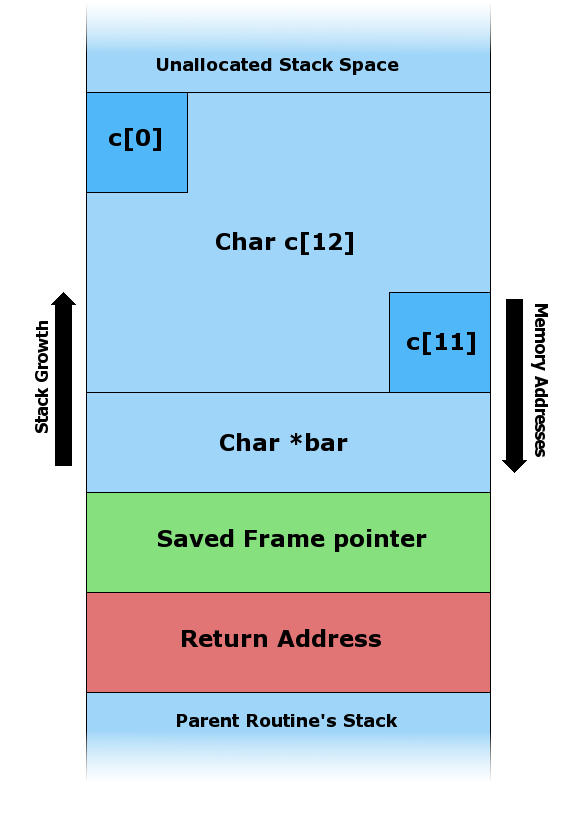
\includegraphics[scale=0.2]{Stack_Overflow_2.png}
     \end{column}
     \begin{column}[T]{4cm} % alternative top-align that's better for graphics
         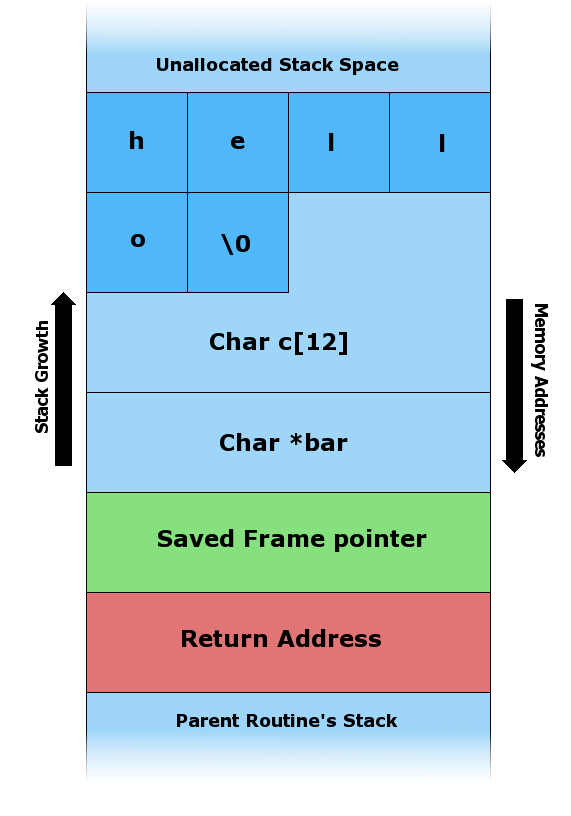
\includegraphics[scale=0.2]{Stack_Overflow_3.png}
     \end{column}
     \begin{column}[T]{6cm} % alternative top-align that's better for graphics
         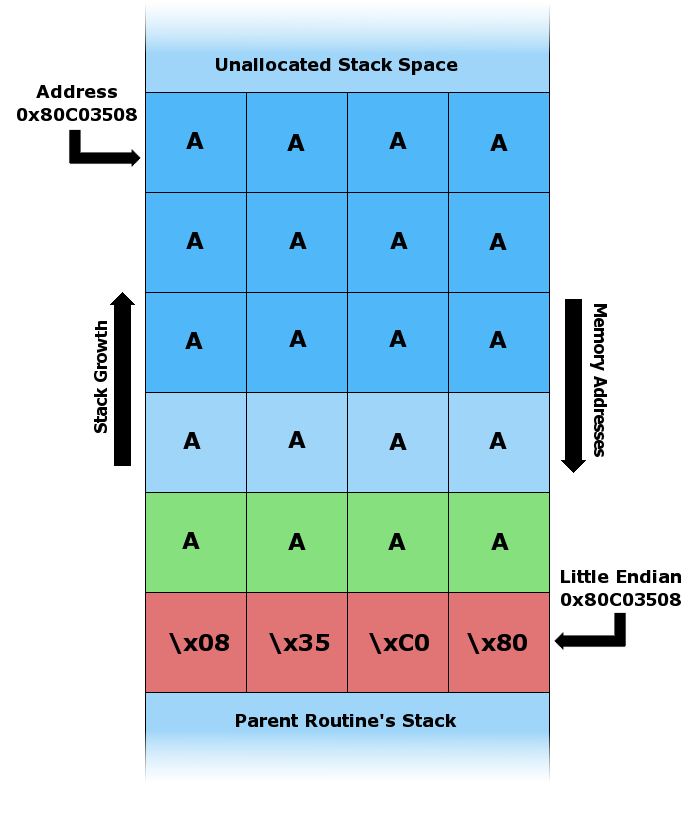
\includegraphics[scale=0.2]{Stack_Overflow_4.png}
     \end{column}
     \end{columns}
\end{frame}

\begin{frame}
\frametitle{Mecanismos de defensa}
\begin{enumerate}
	\item Address Space Layer Randomization.
	\item Data Execution Prevention.
\end{enumerate}
\end{frame}

\section{Llevarlo a la pr\'actica}

\begin{frame}
\frametitle{Intentos de llevarlo a la pr\'actica}
\begin{enumerate}
	\item M\'etodo te\'orico e intrepretaci\'on del c\'odigo.
	\item Depuraci\'on y fuerza bruta.
	\item Combinaci\'on de los dos anteriores.
\end{enumerate}
\end{frame}

\begin{frame}
\frametitle{Desensamblado de sbo}
\begin{block}{sbo.att}
Dump of assembler code for function main:\\
   0x08048320 <+0>:	lea    0x4(\%esp),\%ecx\\
   0x08048324 <+4>:	and    \$0xfffffff0,\%esp\\
   0x08048327 <+7>:	pushl  -0x4(\%ecx)\\
   0x0804832a <+10>:	push   \%ebp\\
   0x0804832b <+11>:	mov    \%esp,\%ebp\\
   0x0804832d <+13>:	push   \%ecx\\
   0x0804832e <+14>:	sub    \$0x4c,\%esp\\
   0x08048331 <+17>:	mov    0x4(\%ecx),\%eax\\
   0x08048334 <+20>:	pushl  0x4(\%eax)\\

   \end{block}
\end{frame}

\begin{frame}
\frametitle{Desensamblado de sbo(2)}
\begin{block}{sbo.att(2)}
   0x08048337 <+23>:	lea    -0x48(\%ebp),\%eax\\
   0x0804833a <+26>:	push   \%eax\\
   0x0804833b <+27>:	call   0x80482f0 <strcpy@plt>\\
   0x08048340 <+32>:	mov    -0x4(\%ebp),\%ecx\\
   0x08048343 <+35>:	xor    \%eax,\%eax\\
   0x08048345 <+37>:	leave  \\
   0x08048346 <+38>:	lea    -0x4(\%ecx),\%esp\\
   0x08048349 <+41>:	ret    \\
End of assembler dump.

   \end{block}
\end{frame}

\begin{frame}
\frametitle{Obtener direcci\'on del buffer}
\begin{block}{sbo\_ebp.c}

\#include <stdio.h>\\
\#include <string.h>\\[0.5cm]
int main(int argc, char *argv[])\{\\
\tab char buffer[64];\\
\tab strcpy(buffer, argv[1]);\\[0.5cm]
\tab void *p;\\
\tab asm(``mov \%\%ebp, \%0``:``=a``(p));\\
\tab printf(``ebp \%p\textbackslash n``, p);\\
\tab return 0;\\
\}
   \end{block}
\end{frame}

\section{Para curiosos}

\begin{frame}
\frametitle{Hazlo t\'u tambi'en}
\begin{enumerate}
	\item Ve a mi \href{https://github.com/jmtorrespalma/}{GitHub} y clona el repositorio.
	\item Aseg\'urate de dar los permisos necesarios.
	\item Aseg\'urate de tener instaladas las librerias de 32 bits de gcc, gdb y un int\'erprete de python 2.
	\item Ejecuta make bof.
	\item Si funciona no tiene m\'erito, porque te lo he hecho yo.
	\item Si no funciona , !`enhorabuena! Ahora intenta solucionarlo.
\end{enumerate}
\end{frame}


\end{document}

